\documentclass{beamer}
\usepackage[utf8]{inputenc}
\usepackage{amssymb}
\usepackage{xcolor}

\title[Nelder-Mead on the Rheology Problem]{Chapter 5 Project: Apply Nelder-Mead to the Rheology Problem}
\author[Matthew, Tyler, and Sarah]{Matthew Saurette, Tyler Weames, and Sarah Wyse}
\institute[Math 462]{Math 462\\ University of British Columbia - Okanagan}
\date{December 2020}
\usetheme{Madrid}
\usecolortheme{seahorse} 
\useinnertheme{rounded}

\begin{document}
\maketitle


%%%%The Rheology Problem
%------------------------------------------------------------------------
\begin{frame}{The Rheology Problem}


\end{frame}

%%%%The NM Algorithm
%-------------------------------------------------------------------------
\begin{frame}{Nelder-Mead Algorithm}
    \centering
    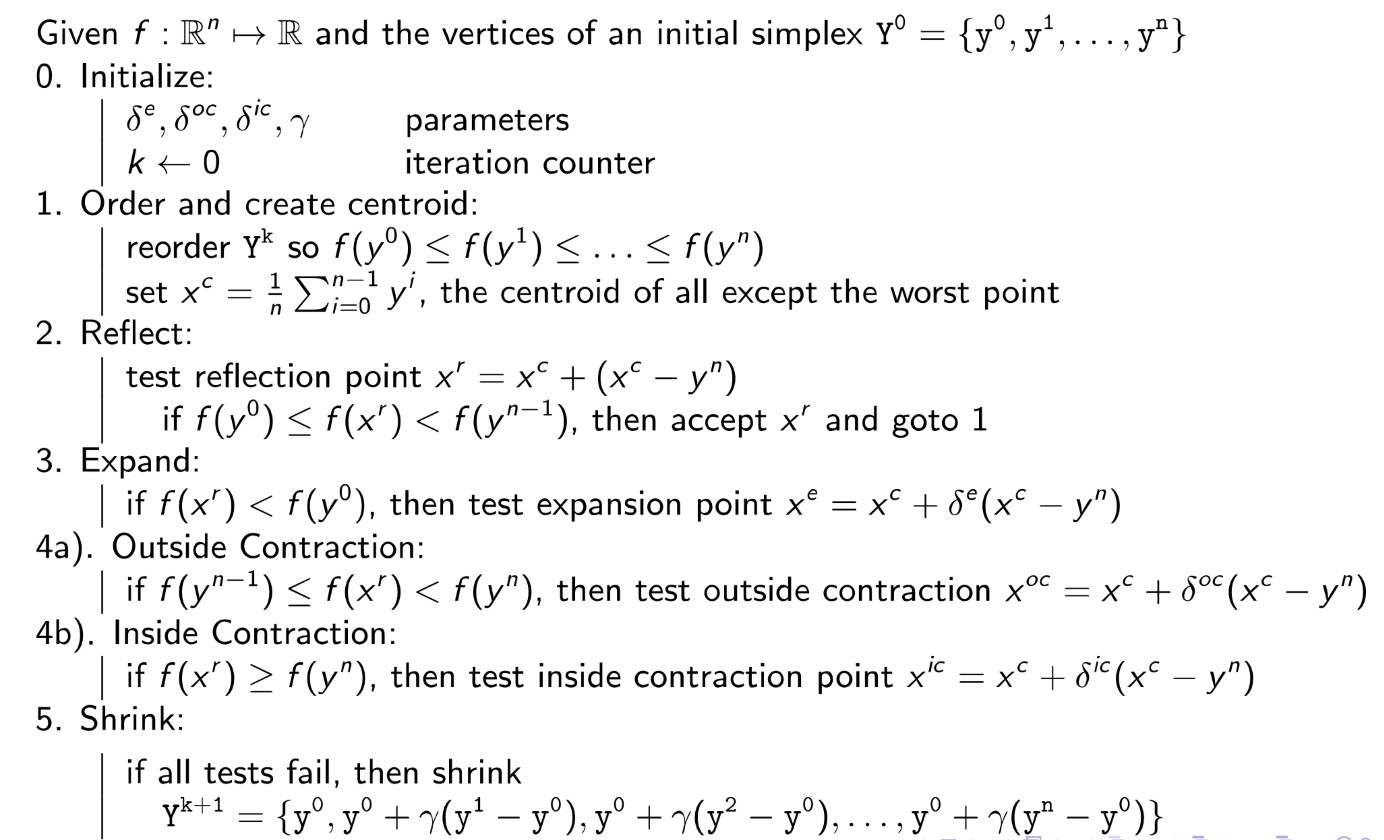
\includegraphics[width=0.95\linewidth]{NMAlgorithm}\\
    \tiny
	\hfill Algorithm from lecture slides    
\end{frame}

\begin{frame}{0. Initialize}
	\centering
	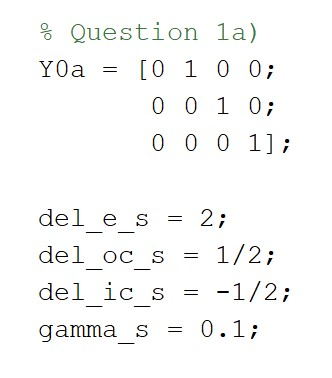
\includegraphics[width=0.35\linewidth]{Initialize}
	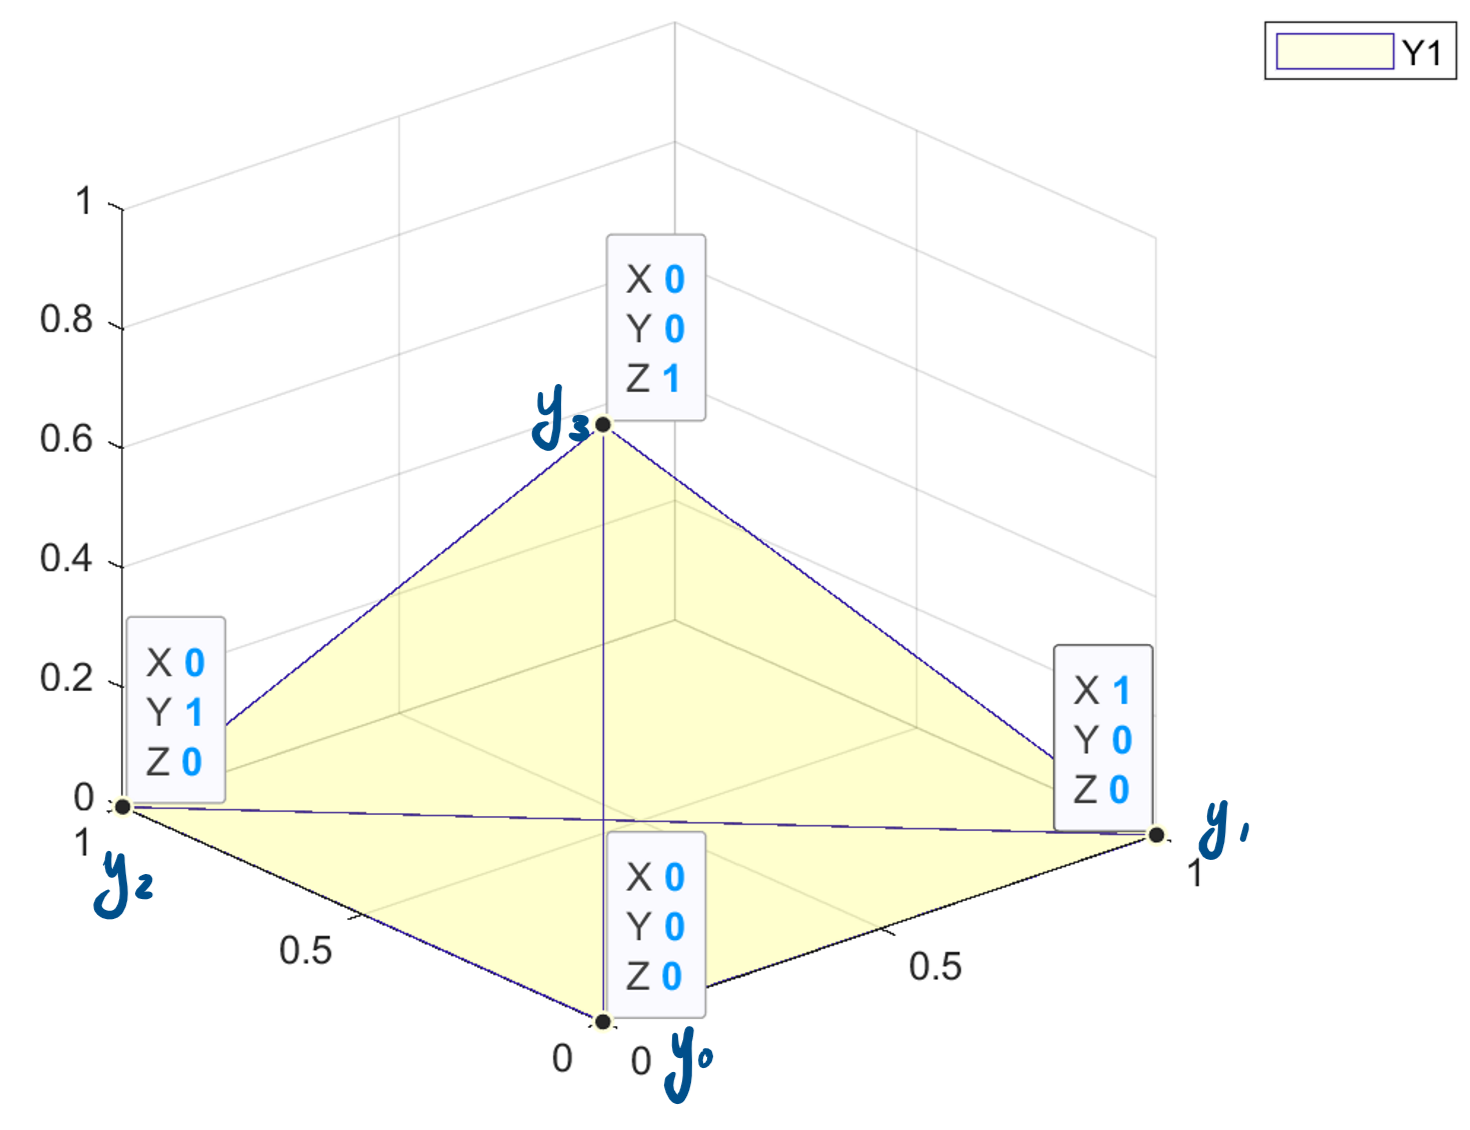
\includegraphics[width=0.59\linewidth]{InitializeFig}
\end{frame}

\begin{frame}{1. Order}
	\begin{columns}
	\begin{column}{0.35\linewidth}
		\centering
		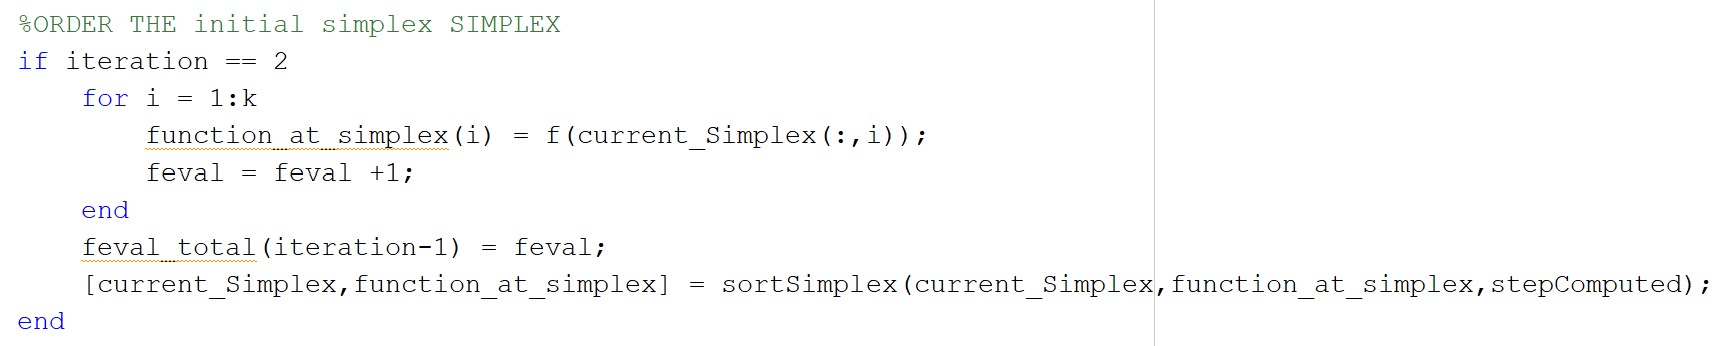
\includegraphics[width=0.95\linewidth]{Order1}
		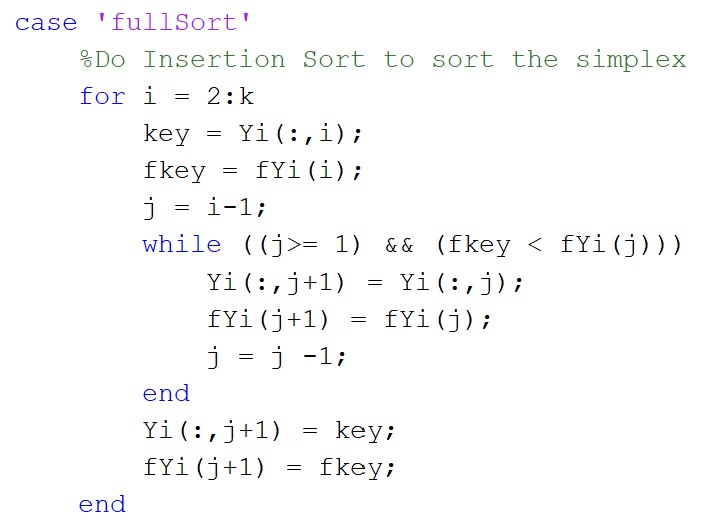
\includegraphics[width=0.95\linewidth]{Shrink2}
	\end{column}
	\begin{column}{0.59\linewidth}
		\centering
		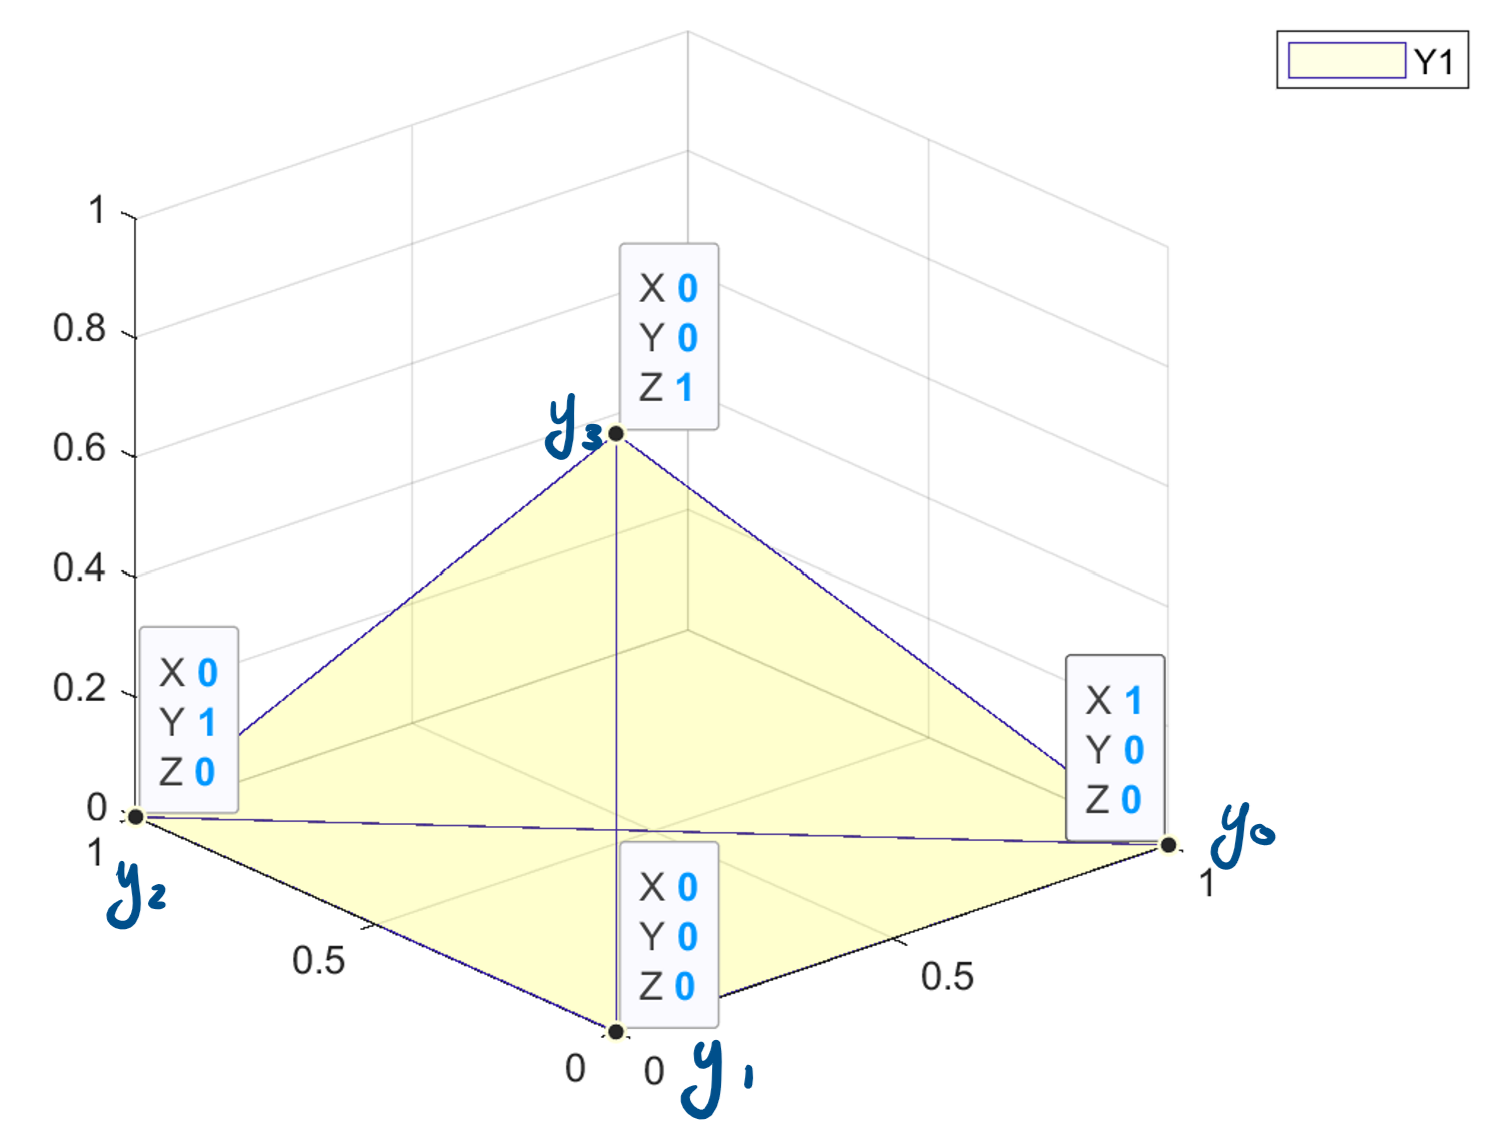
\includegraphics[width=0.95\linewidth]{Order1Fig}
	\end{column}
	\end{columns}
\end{frame}

\begin{frame}{1 and 2. Calculate centroid and $x^r$}
	\begin{columns}
	\begin{column}{0.35\linewidth}
		\centering
		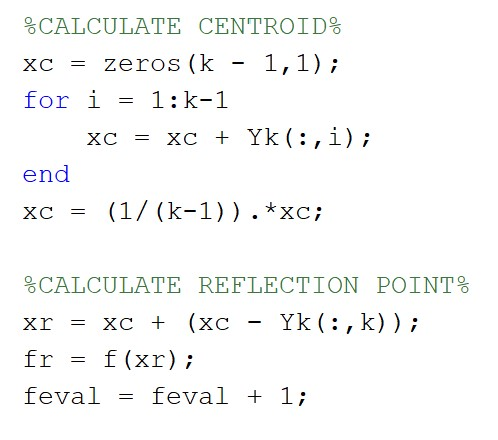
\includegraphics[width=0.95\linewidth]{Order2}
	\end{column}
	\begin{column}{0.59\linewidth}
		\centering
		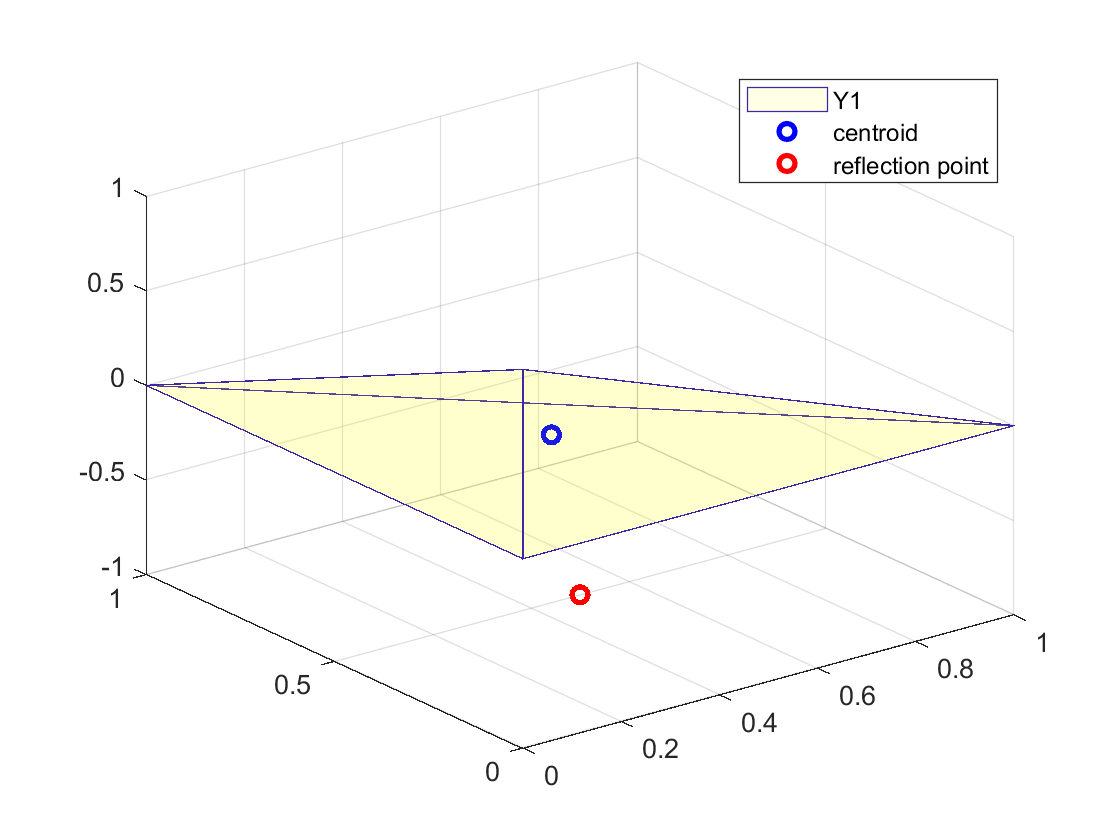
\includegraphics[width=0.95\linewidth]{Order2Fig}
	\end{column}
	\end{columns}
\end{frame}

\begin{frame}{2. Reflect}
	\begin{columns}
	\begin{column}{0.39\linewidth}
		\centering
		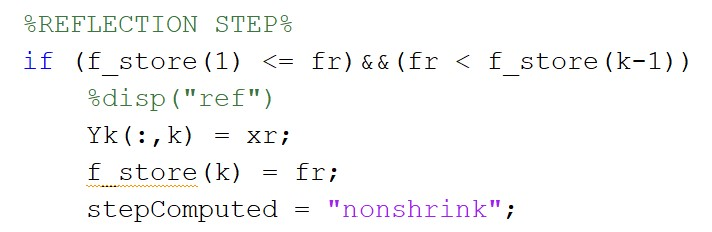
\includegraphics[width=0.95\linewidth]{Reflect}
	\end{column}
	\begin{column}{0.59\linewidth}
		\centering
		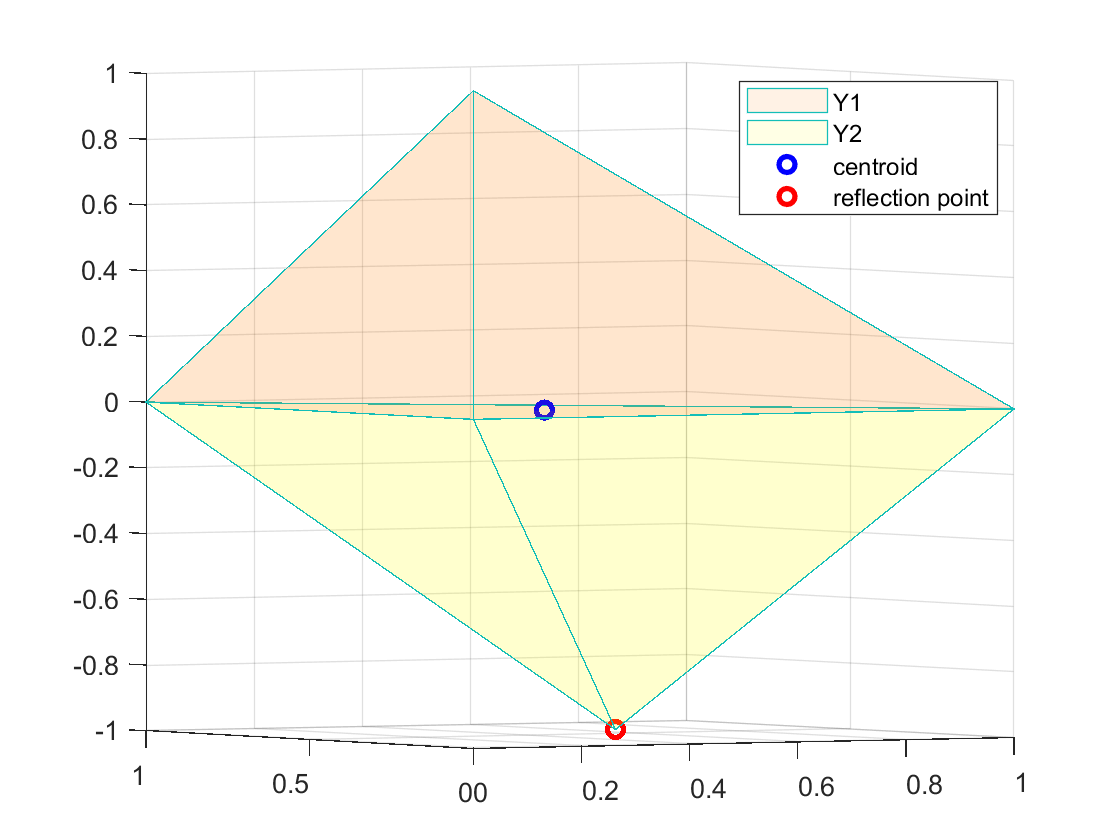
\includegraphics[width=0.95\linewidth]{ReflectFig}
	\end{column}
	\end{columns}
\end{frame}

\begin{frame}{3. Expand}
	\begin{columns}
	\begin{column}{0.39\linewidth}
		\centering
		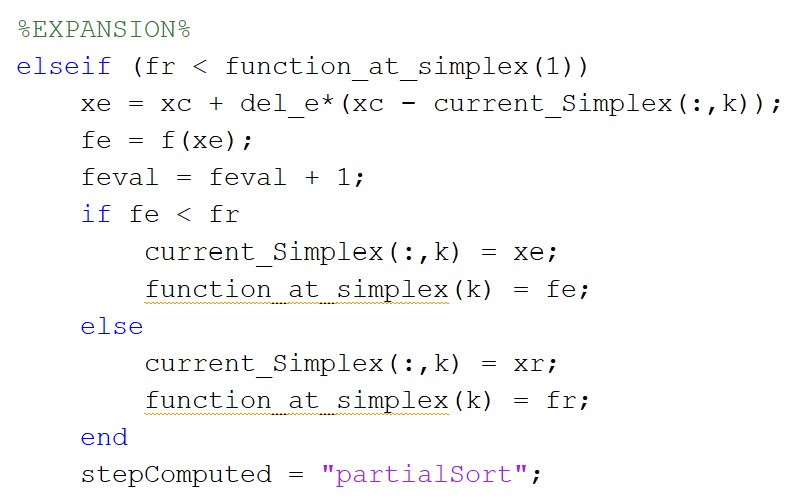
\includegraphics[width=0.95\linewidth]{Expand}
	\end{column}
	\begin{column}{0.59\linewidth}
		\centering
		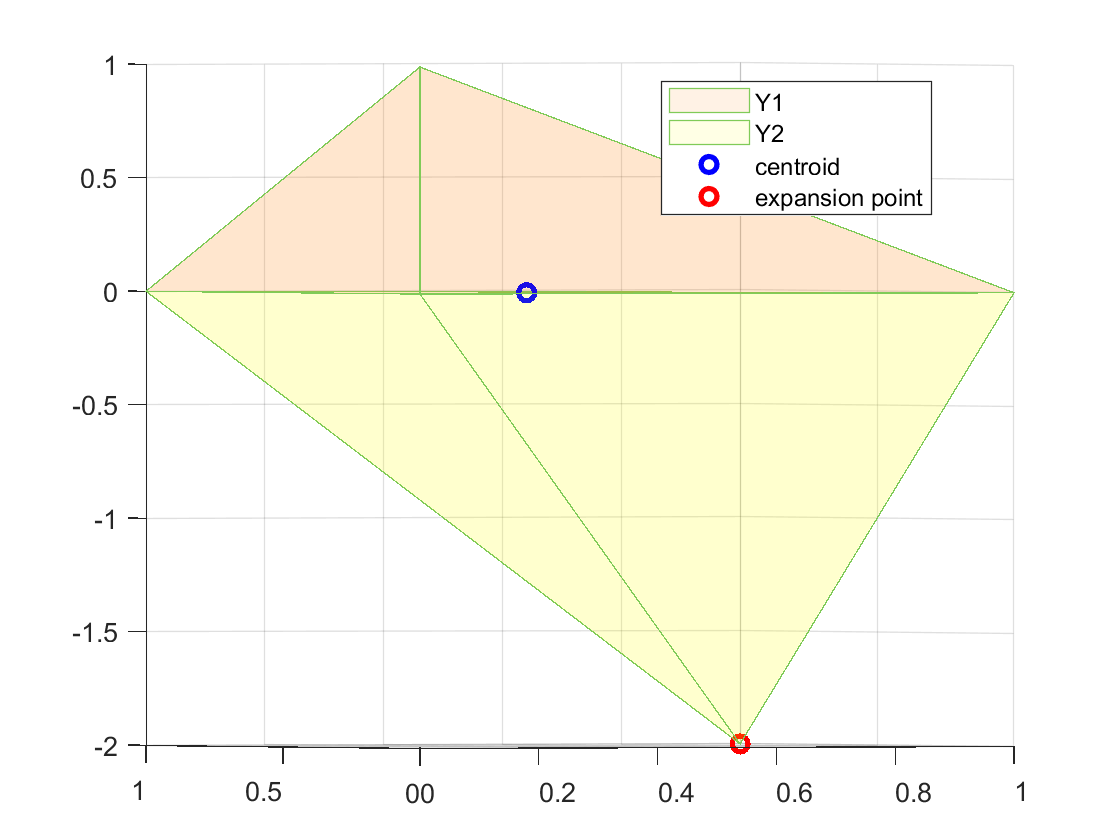
\includegraphics[width=0.95\linewidth]{ExpandFig}
	\end{column}
	\end{columns}
\end{frame}

\begin{frame}{4.a) Outside Contraction}
	\begin{columns}
	\begin{column}{0.39\linewidth}
		\centering
		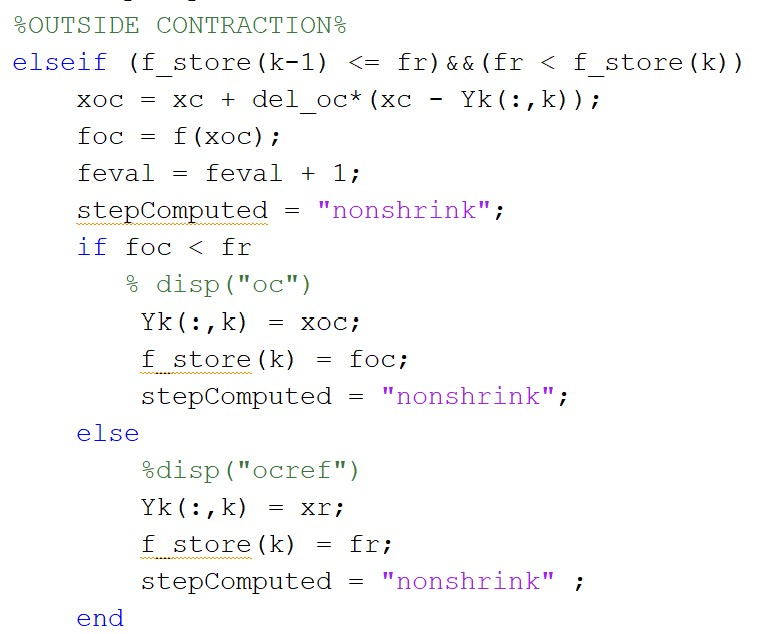
\includegraphics[width=0.95\linewidth]{OC}
	\end{column}
	\begin{column}{0.59\linewidth}
		\centering
		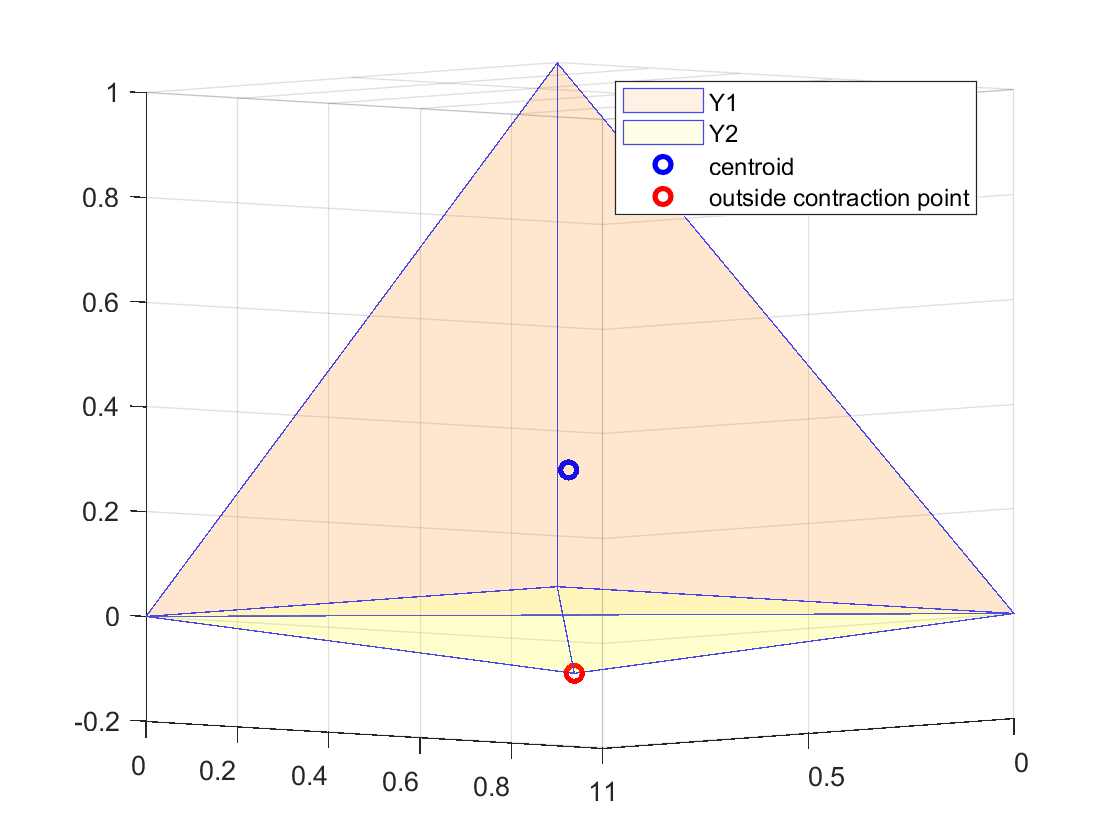
\includegraphics[width=0.95\linewidth]{OCFig}
	\end{column}
	\end{columns}
\end{frame}

\begin{frame}{4.b) Inside Contraction}
	\begin{columns}
	\begin{column}{0.39\linewidth}
		\centering
		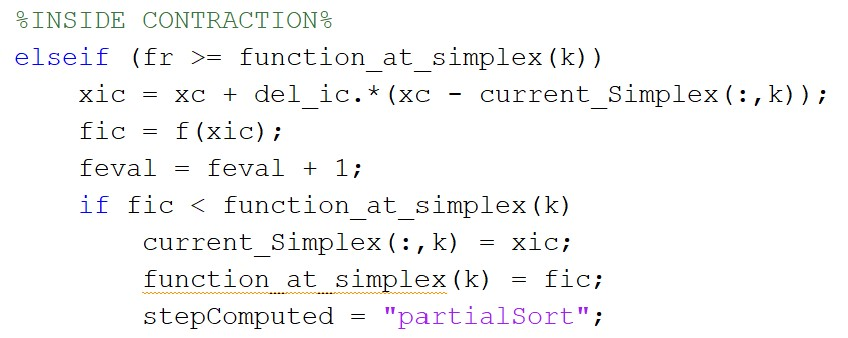
\includegraphics[width=0.95\linewidth]{IC}
	\end{column}
	\begin{column}{0.59\linewidth}
		\centering
		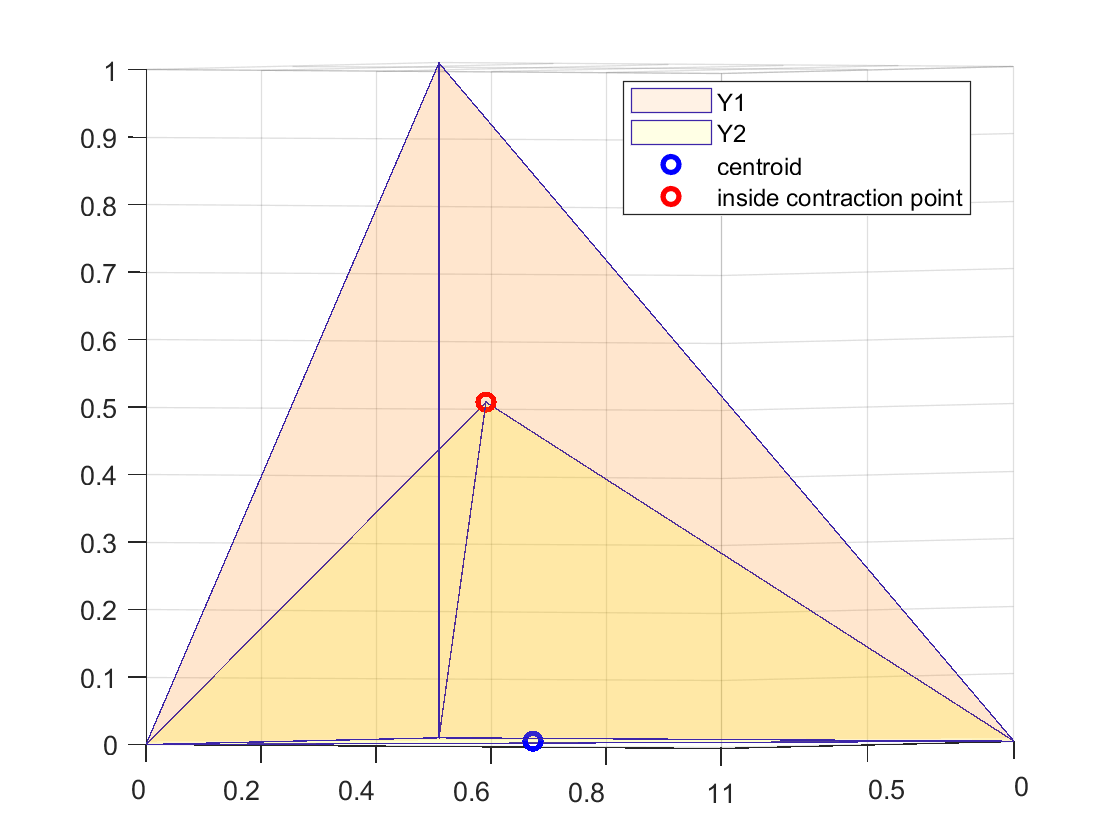
\includegraphics[width=0.95\linewidth]{ICFig}
	\end{column}
	\end{columns}
\end{frame}

\begin{frame}{5. Shrink}
	\begin{columns}
	\begin{column}{0.39\linewidth}
		\centering
		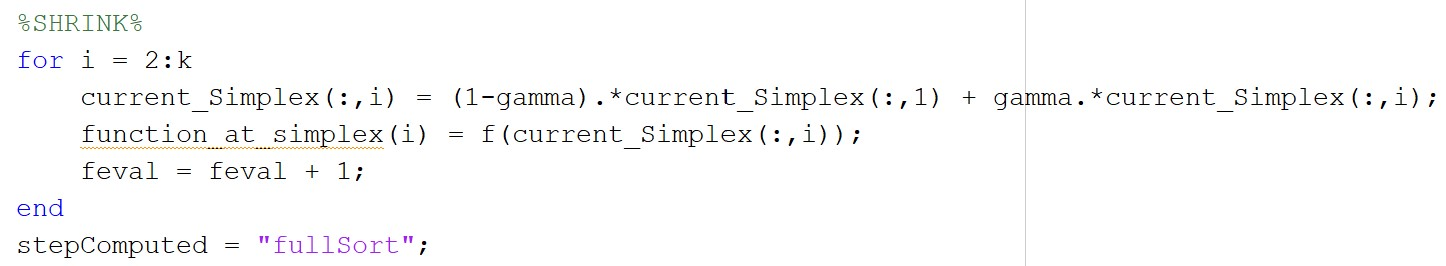
\includegraphics[width=0.95\linewidth]{Shrink}
		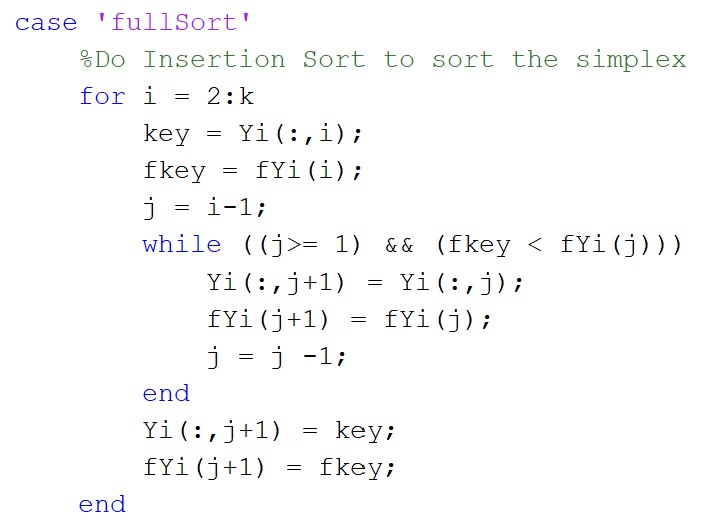
\includegraphics[width=0.85\linewidth]{Shrink2}
	\end{column}
	\begin{column}{0.59\linewidth}
		\centering
		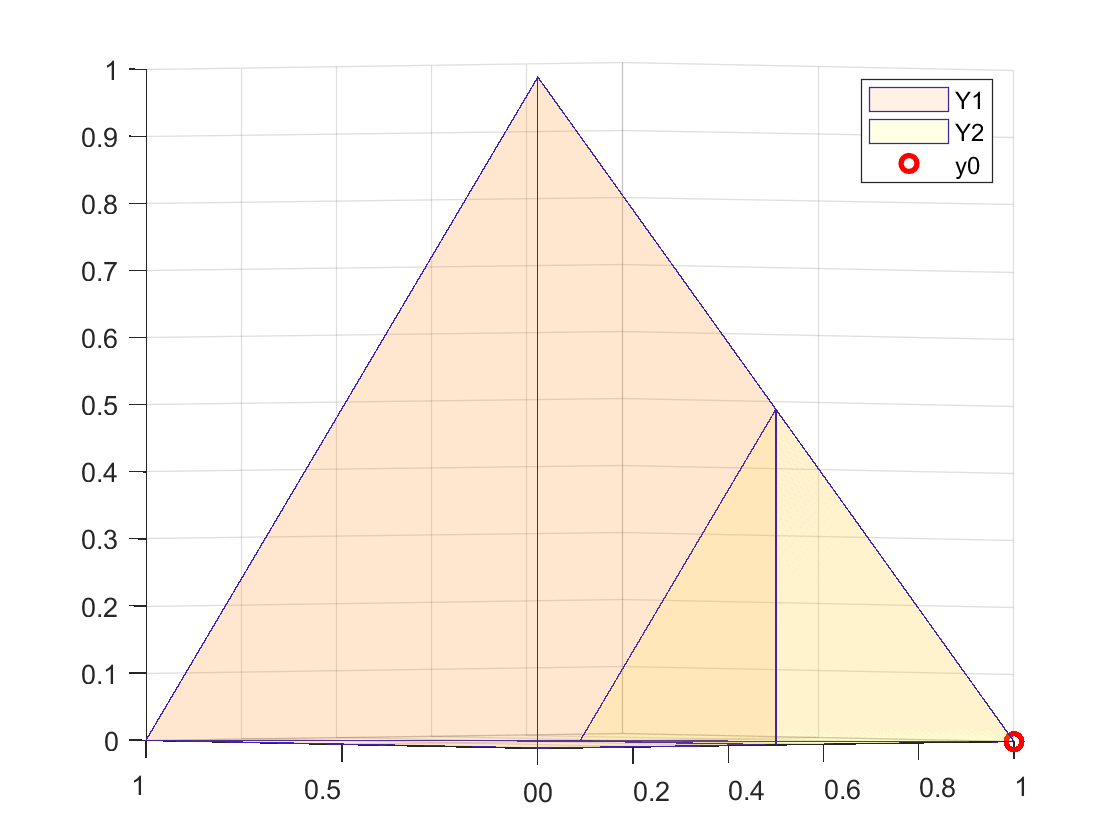
\includegraphics[width=0.95\linewidth]{ShrinkFig}
	\end{column}
	\end{columns}
\end{frame}

%%%%Examples
%------------------------------------------------------------------------



%%%%Solve the Rheology Problem
%------------------------------------------------------------------------




\end{document}